\chapter{Requirements Elicitation}
\label{chap:requirements}

In this chapter the functional and non-functional requirements will be presented.

``A software requirement is a capability needed by the user to solve a problem or to achieve an objective. In other words, requirement is a software capability that must be met or possessed by a system or system component to satisfy a contract, standard, specification, or other formally imposed documentation. Ultimately, what we want to achieve is to develop quality software that meets customers' real needs on time and within budget.'' \parencite{req}.

The project high-level goal was well defined since the start:

Develop an IoT Platform with focus on extensibility to decrease the delivery time of new business cases and allow others to implement their business on top of the platform.

The definitive business cases to develop changed various times during the project lifespan due to intricate contract promises with third parties that never ended up seeing the light of day. The business cases, ordered by the first time they were requested, and grouped by organization, can be summarized in Table~\ref{tab:requirements:servicerequests}.

These business cases can be vaguely characterized according to the following organization's needs:

\begin{itemize}
    \item \textbf{Deployment Environment}: Should the solution be deployed on-premise or in the cloud;
    \item \textbf{Multi-Tenancy}: Should the organization share an instance of the solution with others or not (according \cite{multi});
    \item \textbf{Data Shareability}: Does the organization wants to provide their data to the public (according to \cite{pra2.2017.14505401085});
    \item \textbf{Information Access and Visualization}: Where and how to present and serve information. Present information visually in the costumer organization platform, directly in this solution or via other means such as a simple \gls{API}, SMS, or email.
\end{itemize}

\begin{table}[H]
    \caption[Summary of the main requirements of the requested business cases]{Summary of the main requirements of the requested business cases}
    \label{tab:requirements:servicerequests}
    \centering
    \small
    \begin{tabular}{@{}ccllll@{}}
    \toprule
    \textbf{Org} &
      \textbf{Business Case} &
      \textbf{\begin{tabular}[c]{@{}l@{}}Deployment\\Environment\end{tabular}} &
      \textbf{\begin{tabular}[c]{@{}l@{}}Multi-\\Tenancy\end{tabular}} &
      \textbf{\begin{tabular}[c]{@{}l@{}}Data \\Shareability\end{tabular}} &
      \textbf{\begin{tabular}[c]{@{}l@{}}Information \\ Access and \\Visualization\end{tabular}} \\ \midrule
    \multirow{5}{*}{A} & Fleet Management           & On-Premise & Single-Tenant & Private & Sensae Console     \\ \cmidrule(l){2-6}
                       & Smart Irrigation           & On-Premise & Single-Tenant & Private & Sensae Console     \\ \cmidrule(l){2-6}
                       & Smart Parking              & On-Premise & Single-Tenant & Private & Sensae Console     \\ \cmidrule(l){2-6}
                       & Indoor Fire Detention      & On-Premise & Single-Tenant & Private & SMS and Email      \\ \cmidrule(l){2-6}
                       & Public Health Surveillance & On-Premise & Single-Tenant & Public  & Sensae Console     \\ \midrule
    B                  & Fleet Management           & Cloud      & Single-Tenant & Private & Org B Platform     \\ \midrule
    \multirow{3}{*}{C} & Smart Irrigation           & Cloud      & Multi-Tenant    & Private & Sensae Console     \\ \cmidrule(l){2-6}
                       & Indoor Fire Detention      & Cloud      & Multi-Tenant    & Private & SMS and Email      \\ \cmidrule(l){2-6}
                       & Chicken Farm Monitoring    & Cloud      & Multi-Tenant    & Private & Sensae Console     \\ \midrule
    D                  & Smart Irrigation           & Cloud      & Multi-Tenant    & Private & Sensae Console     \\ \bottomrule
    \end{tabular}
\end{table}

The requirements detailed in the following sections were founded on top of the requested business cases mentioned above. These requirements were constantly tailored according to the latest talks with the third parties involved. Even though many requested business cases weren't implemented, they guided the author to the design and development of the final solution, \textbf{Sensae Console} and \gls{PoC}s.

At the time of writing, the \gls{PoC}s developed answer three business cases: (i) Fleet Management, (ii) Smart Irrigation and (iii) Indoor Fire Detention. The other business cases were either abandoned or requested too close to the writing of this dissertation and therefore will not be detailed.

\section{Functional Requirements}
\label{sec:requirements:functional}

Functional Requirements define the user-faced functionalities/operations that the solution to develop must support in the future.

According to \cite{van2009requirements}, ``Functional requirements define the functional effects that the software-to-be is required to have on its environment. The effects characterized by such requirements result from operations to be automated by the software. Functional requirements may also refer to environmental conditions under which operations should be applied.''

The following sections describe the requirements associated with each role inside \textbf{Sensae Console}, the solution that this project aims to deliver, and the \gls{PoC}s developed, refereed as \textbf{Business Applications}.

\subsection{Roles}
\label{subsec:requirements:functional:roles}

The meetings that took place during this project's time span lead to the definition of three main roles:

\begin{itemize}
    \item \textbf{Manager}: a role with full control over the \textbf{Sensae Console} and all its data. He/She has also full control of all \textbf{Business Applications};
    \item \textbf{Costumer}: a role with restricted control over \textbf{Sensae Console}, controlling only the devices, employees and departments registered under his/her own organization. He/She has access to the requested \textbf{Business Applications};
    \item \textbf{Anonymous User}: a role with no account in the system. He/She has access to the publicly available \textbf{Business Applications} and data feed from \textit{'public'} devices in the system.
\end{itemize}

Apart from the basic costumer requirements inside \textbf{Sensae Console}, each \textbf{Business Application} has specific use cases that will be detailed in the section~\ref{subsubsec:requirements:functional:sensae:costumer}.

Essentially, the difference between these roles boils down to what permissions each has and the extent of data each one can visualize. The Section~\ref{subsubsec:design:domain:bounded_contexts:identity} details how this is handled by the solution.

The following sections will be divided in:

\begin{itemize}
    \item Sensae Console: presenting the functional requirements associated with each role;
    \item Business Applications: presenting the functional requirements associated with each business case supported.
\end{itemize}

\subsection{Sensae Console}
\label{subsec:requirements:functional:sensae}

The idea behind Sensae Console functional requirements boils down to the core functionalities it should provide so that creating and maintaining business applications is simplified.

The Anonymous User role is disregarded here since his/her goal is to simply benefit from curated and publicly available information provided by the business applications.

\subsubsection{Manager}
\label{subsubsec:requirements:functional:sensae:manager}

The purpose of the Manager is to supervise an instance of \textbf{Sensae Console} and its costumers. This role is an extension of the Costumer role and can do and see everything a Costumer can. A Manager is assign to an instance of \textbf{Sensae Console} at creation time and belongs to the highest domain, the \textit{Root Organization} as described in Section~\ref{subsubsec:design:domain:bounded_contexts:identity}.

The following list documents the functional requirements related to this actor regarding the \textbf{Sensae Console} administration:

\begin{enumerate}
    \item The Manager must be able to create, view, update and delete device payload decoders;
    \item The Manager must be able to create, view, update and delete device payload processors (or mappers);
    \item The Manager must be able to create, view, update and delete rules that trigger alerts;
    \item The Manager must be able to define, view, update and remove device specific information;
    \item The Manager must be able to define the permissions of any organization;
    \item The Manager must be able to assign new devices to a specific organization;
    \item The Manager must be able to assign new authenticated users to a specific organization.
\end{enumerate}

As described in Sections~\ref{subsubsec:design:domain:bounded_contexts:processor} and ~\ref{subsubsec:design:domain:bounded_contexts:decoder}, the decoders and processors referenced in the first and second items are meant to translate unsanitized device data. This is highly required since ``the nonexistence of interoperability standards is one of \gls{IoT}'s most pressing issues, (...) designing a system using the latest available standard proposal does not ensure its adoption or that the standard will be deprecated before the system reaches the market'' - \cite{DIAS2022100529}.

The rules referenced in the third item can be used to program how the system answers to certain abnormal occurrences, more context is given in Section~\ref{subsubsec:design:domain:bounded_contexts:rule}.

The device information mentioned in item four is detailed in Section~\ref{subsubsec:design:domain:bounded_contexts:device}.

Even though the first four groups of operations belong to the Manager role, they can be assigned to normal Costumers on special occasions. As an example, the Organization A and B referenced in Table~\ref{tab:requirements:servicerequests}, had employees capable of fully managing the solution and wanted an instance of \textbf{Sensae Console} exclusively for them. This meant that, when given access to these operations, there was a lower risk for them to misconfigure the platform due to a lack of knowledge and no risk to interfere with other Organizations' data pipeline, since they were the only ones in that instance.

\subsubsection{Costumer}
\label{subsubsec:requirements:functional:sensae:costumer}

The purpose of a Costumer is to manage his/her own organizations.
The following list documents the universal functional requirements related to this role:

\begin{enumerate}
    \item A Costumer must be able to create and remove a department under his/her organization;
    \item A Costumer must be able to define the permissions for all other Costumers in a department under his/her organization;
    \item A Costumer must be able to assign and move another Costumer from/to a department under his/her organization;
    \item A Costumer must be able to move a sensor from one department to another department under his/hers organization.
\end{enumerate}

\subsection{Business Applications}
\label{subsec:requirements:functional:services}

This section describes the functional requirements associated with each business application needs from the point of view of a costumer.

The Anonymous User role was created to answer organization A concerns regarding the Public Health Surveillance business case. The business application should be available for the public to consult the current and past \gls{AQI} levels measured in the city without needing to create an account. Even though this business case was abandoned, the Anonymous User role was integrated in the solution.

Each supported business application has specific use cases defined below.

\subsubsection{Fleet Management}
\label{subsubsec:requirements:functional:services:fleet}

Within a simple Fleet Management business case the major utilities a Costumer can benefit from are: (i) real-time tracking of his vehicles and (ii) visualizing past data regarding the whereabouts of his fleet. A more advanced Fleet Management would for example provide \gls{KPI} reports about the fleet or alerts when a vehicle would enter or leave a geofence. This advanced topics were mentioned by organization A close to the day when they withdrawn the contract and therefore were never implemented.

The following list documents the key functional requirements of this business case as prescribed by the third parties:

\begin{enumerate}
    \item A Costumer must be able to track in real-time a vehicle location and motion status;
    \item A Costumer must be able to see the itineraries of a vehicle in defined time span;
    \item A Costumer must be able to see where, when and for how long a vehicle was parked;
    \item A Costumer must be able to see the traveled distance of a vehicle, in a defined time span.
\end{enumerate}

This business case' concepts are discussed with more detail in Section~\ref{subsubsec:design:domain:bounded_contexts:fleet}.

\subsubsection{Indoor Fire Detention}
\label{subsubsec:requirements:functional:services:fire}

An Indoor Fire Detention system usual main objective is to trigger an alarm when precarious conditions are meet. As a first milestone, both companies, A and C, requested a simple alarm system with no other features. Features such as data retention, data visualization and continuous camera vigilance were later requested. As such, the only requirement related to this business case is:

\begin{enumerate}
    \item A Costumer must be able to receive alerts regarding critical conditions that may indicate a fire outbreak, either via SMS or email.
\end{enumerate}

\subsubsection{Smart Irrigation}
\label{subsubsec:requirements:functional:services:irrigation}

Within a Smart Irrigation business case the major utilities a Costumer can benefit from are: (i) real-time tracking of a garden/greenhouse conditions, (ii) archiving conditions for later use/consulting and (iii) activate/deactivate the irrigation system remotely.

The following list documents the key functional requirements related to this business case as prescribed by the third parties:

\begin{enumerate}
    \item A Costumer must be able to manage his/her garden's information;
    \item A Costumer must be able to track a gardens' conditions in real-time;
    \item A Costumer must be able to see past conditions of a garden;
    \item A Costumer must be able to activate and deactivate the irrigation system remotely.
\end{enumerate}

The concepts surrounding this business case are discussed with more detail in Section~\ref{subsubsec:design:domain:bounded_contexts:irrigation}.

\section{Non Functional Requirements}
\label{sec:requirements:non_functional}

Non-functional requirements define constraints on software development, maintenance, and allocation.
According to \cite{van2009requirements}, “Non-functional requirements define constraints on the way the software-to-be should satisfy its functional requirements or on the way it should be developed.”

This analysis used the FURPS+ model \parencite{eeles2005capturing}, which distributes the non-functional requirements into the following categories: functionality, usability, reliability, performance, supportability, design requirements, implementation requirements, interface requirements and physical requirements. Some of the requirements here presented were extrapolated from the ones mentioned by \cite{iot-a} and therefore reference their \textit{UNI ID}.

Each category's requirements are presented in the following sections.

\subsection{Functionality Requirements}
\label{subsec:requirements:non_functional:functionality}

Regarding the Functionality category, the following requirements were identified:

\begin{enumerate}
    \item User Authentication: Apart from the Anonymous Users, everyone else must be authenticated to use the system;
    \item User Authorization: Everyone only has access to what his/her permissions cover, the system shall provide different access permissions to information (UNI.067);
    \item Data Exposure Control: Users have control how their data is exposed to (Single-Tenant with) other users (UNI.002);
    \item Communication: The system shall support event-based, periodic, and/or autonomous communication (UNI.005);
    \item Autonomicity: The system shall enable autonomous goal-driven (task-driven) collaboration between devices or services (UNI.010);
    \item Data parameterization: The system shall provide a resolution infrastructure for naming, addressing and assignment of virtual entities and services (UNI.030);
    \item Data Storage: The system shall provide historical information about the \gls{IoT} device (physical entity) (UNI.041);
    \item Security in Communication: The use of secure protocols between clients and the system is mandatory, e.g.: https instead of http;
    \item Security in User-provided code: All user-provided code must run in sandbox's to prevent permission escalation, data theft and other related concerns;
    \item Data Analysis: The system shall support the integration with a \gls{CEP} component (UNI.232);
    \item Data Filtering: The system shall be able to filter erroneous sensor data (e.g. GPS location coordinates of a land vehicle appearing in the middle of the ocean;
    \item Real-time Alerts: The system must notify the interested clients in real time of any alarm triggered by custom rules;
    \item Real-Time Information: Any change to the system must be notified to the client in real-time without resorting to techniques like automatic/manual polling. This includes new sensor data, changes to virtual devices, alarms/rules definitions, decoders and anything else deemed important.
\end{enumerate}

\subsection{Usability Requirements}
\label{subsec:requirements:non_functional:usability}

Since this project is a greenfield and is still in the early stages of conception, the Usability category is not a major concern. No requirements were proposed.

\subsection{Reliability Requirements}
\label{subsec:requirements:non_functional:reliability}

The Reliability category has the following requirements:

\begin{enumerate}
    \item The system must validate all user inputs, denying code injection according to \cite{top10};
    \item The system must be able to recover from a failure state such as a crash in the system or any system component;
    \item The system shall provide availability through resilience (UNI.064);
    \item The system must identify or protect itself against compatibility errors due to versions mismatches between the system and third-party scripts or components, e.g. a valid rule in the system version 1 may not be compatible with the system version 2; if that is the case the system should inform the Costumer and not use the rule.
\end{enumerate}

\subsection{Performance Requirements}
\label{subsec:requirements:non_functional:performance}

Even though this work is in its early stages of development, the performance of the system is a priority. For single-tenant instances, the requirements specified for this category are:

\begin{enumerate}
    \item When a new and valid device data is received, the system should make this information available to any user within 2 seconds in 90\% of the cases. The time for the information to be presented should never exceed 5 seconds unless the network connection is broken (in which case the user should be notified);
    \item When an alarm is triggered, the system should dispatch the alarm within 10 seconds in 90\% of the cases;
    \item Concurrent Utilization: The system must be able to be used by various users at the same time;
    \item High Data Ingestion: The system must be able to successfully process, evaluate and store device data with a throughput of at least 5000 data units per minute.
\end{enumerate}

\subsection{Supportability Requirements}
\label{subsec:requirements:non_functional:supportability}

In the Supportability category the following requirements were identified:

\begin{enumerate}
    \item The system must be highly configurable so that support for any type of device, specially payload decoding, can be added without the need for restarting/rebuilding it;
    \item The system must be agnostic to cloud computing platforms and be independent of any service provided by cloud computing platforms. This ensures that it can be deployed on-site or on a single cloud computing platform;
    \item The system must provide simple methods to integrate business applications that answer new business cases without the need to rebuilding it;
    \item The system shall be extensible for future technologies (UNI.093);
    \item The system must attempt to be agnostic to \gls{IoT} middleware platforms, being able to exchange data with most of them without the need to restarting/rebuilding it. At least \citetitle{helium} has to be supported.
\end{enumerate}

\subsection{Design Requirements}
\label{subsec:requirements:non_functional:design}

The Design Requirements identified are related to how \textbf{Sensae Console} must interact with External Systems, namely \gls{IoT} middlewares and Identity Providers. This requirements also describe what \gls{API} should be served to Costumers, Organizations and \textbf{Business Applications}.

\begin{figure}[H]
    \centering
    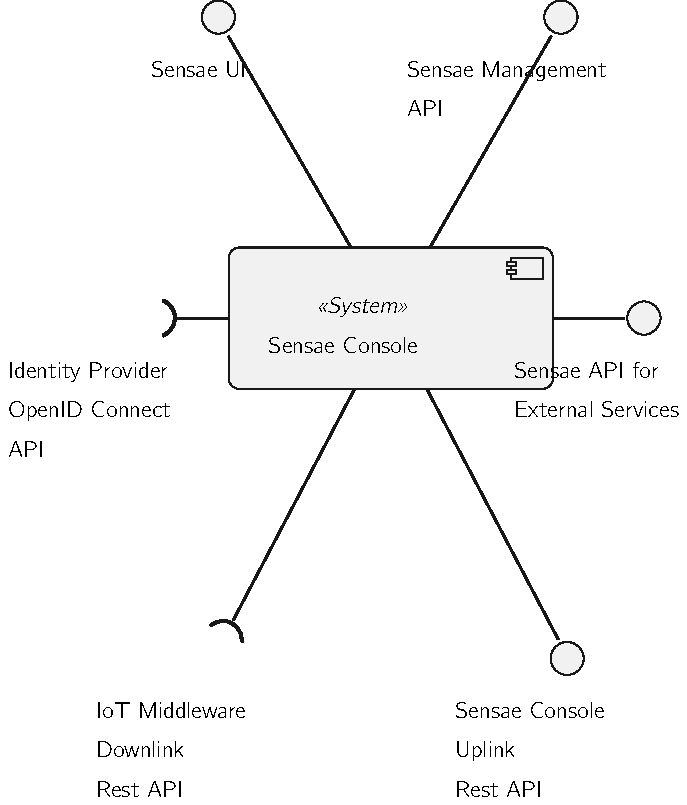
\includegraphics[page=1,width=0.5\columnwidth]{assets/diagrams/design/architectural/level1/logical-view-v2.pdf}
    \caption[Design Requirements Diagram]{Design Requirements Diagram}
    \label{fig:requirements:non_functional:design}
\end{figure}

Most Identity Providers adhere to the OpenID Connect Standard, therefore it's possible to develop a single solution that can exchange information with various Identity Providers in a agnostic manner.
The \textit{'\gls{IoT} Middleware Downlink Rest API'} may require a different implementation for each \gls{IoT} Middleware since there is no Standard that these platforms can follow, according to \cite{KOO20224191}.  

\subsection{Implementation Requirements}
\label{subsec:requirements:non_functional:implementation}

In the Implementation category, the system's shall provide \gls{SPA} for end users to interact with.

\subsection{Interface Requirements}
\label{subsec:requirements:non_functional:interface}

In the Interface category, the following requirements for \textbf{Sensae Console} were identified:

\begin{enumerate}
    \item The system shall require user authentication via OpenID Connect Protocol offered by any Identity Provider;
    \item The system shall support the dispatch of downlinks to devices using, at least, the \citetitle{helium};
    \item The system shall support the ingestion of uplinks from devices using, at least, the \citetitle{helium}.
\end{enumerate}

As for the \textbf{Business Applications}:

\begin{enumerate}
    \item The Indoor Fire Retention related Business Application shall support the dispatch of emails using \gls{SMTP};
    \item The Indoor Fire Retention related Business Application shall support the dispatch of messages using \gls{SMS}.
\end{enumerate}

\subsection{Physical Requirements}
\label{subsec:requirements:non_functional:physical}

In the Physical category, the following requirements were identified:

\begin{enumerate}
    \item The multi-tenant, cloud deployed instance must be publicly available under a single \gls{FQDN};
    \item The system shall be deployed in machines running a Linux kernel;
    \item The various system components shall be containerized using docker;
    \item The various system components shall be orchestrated using docker-compose or kubernetes.
\end{enumerate}

\section{Synopsis}
\label{subsec:requirements:synopsis}

This chapter mentioned the functional requirements of the project defined during its lifespan. This requirements addressed the needs of the various shareholders, divided in three major roles: (i) manager, (ii) costumer and (iii) anonymous user. While the focus of the project lays in supporting common functionalities of \gls{IoT} related services within \textbf{Sensae Console}, this chapter also mentioned the \textbf{Business Applications} requested by third-parties, and their specific requirements.

Although more vague, the non-functional requirements of the project were also presented using the FURPS+ model.

These requirements lead to the solution's design, presented in the next chapter.
